% Appendix Template

\chapter{Instrucciones} % Main appendix title

\label{App_Inst} % Change X to a consecutive letter; for referencing this appendix elsewhere, use \ref{AppendixX}

A continuación se presentan una serie de capturas de pantalla donde se presentan las instrucciones proporcionadas a los participantes en cada uno de los Experimentos realizados.

\textbf{1. Pantalla de bienvenida}

\begin{figure}[th]
\centering
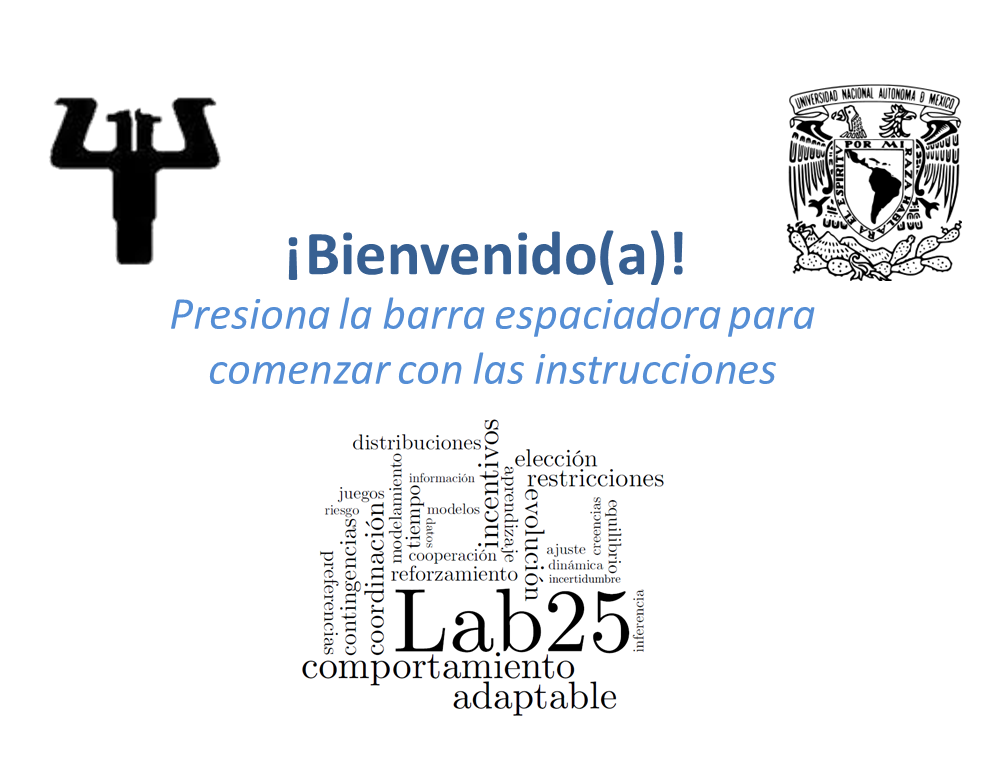
\includegraphics[width=0.95\textwidth]{Figures/Inst_Bienvenido} 
\decoRule
\caption[Pantalla de Bienvenida]{}
\label{fig:csv}
\end{figure}


\textbf{2. Presentación de la tarea principal}

\begin{figure}[th]
\centering
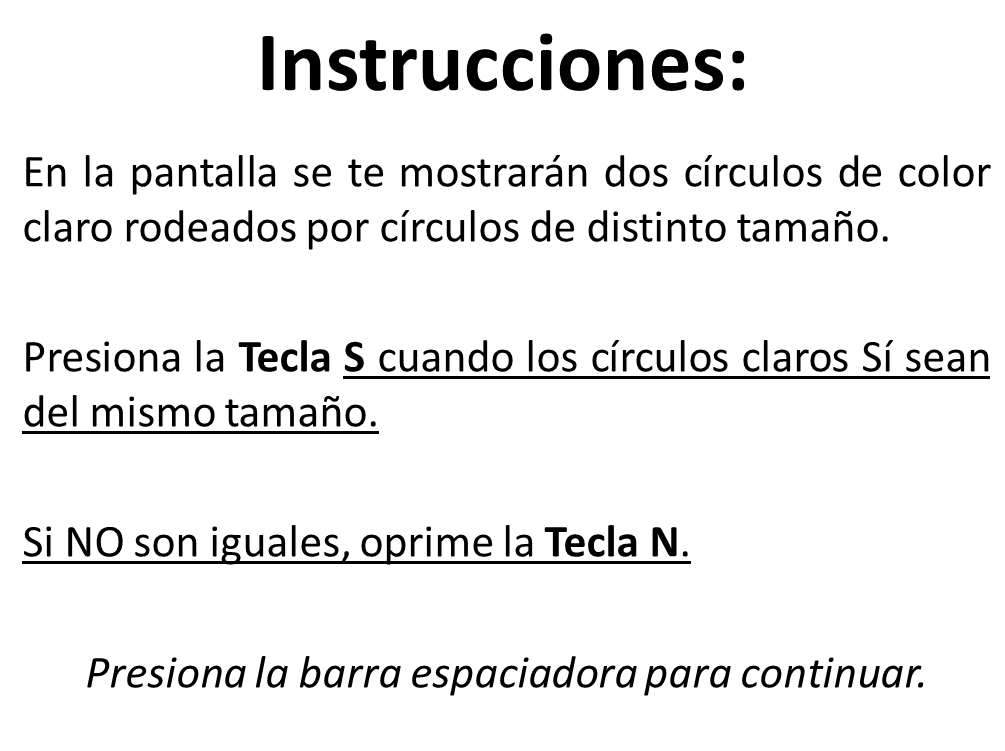
\includegraphics[width=0.95\textwidth]{Figures/Inst_1} 
\decoRule
\caption[Pantalla de Bienvenida]{}
\label{fig:csv}
\end{figure}

\textbf{3. Presentación de un ejemplo}

\begin{figure}[th]
\centering
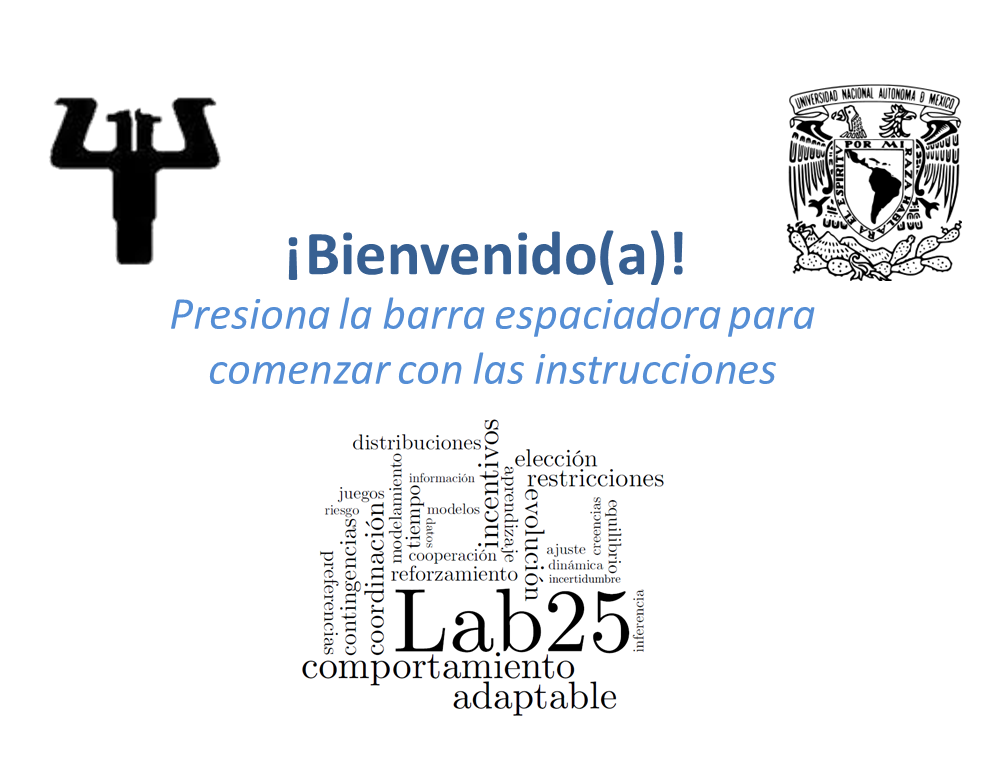
\includegraphics[width=0.95\textwidth]{Figures/Inst_Bienvenido} 
\decoRule
\caption[Pantalla de Bienvenida]{}
\label{fig:csv}
\end{figure}

\textbf{4. Presentación de la tarea de escala de confianza}

\begin{figure}[th]
\centering
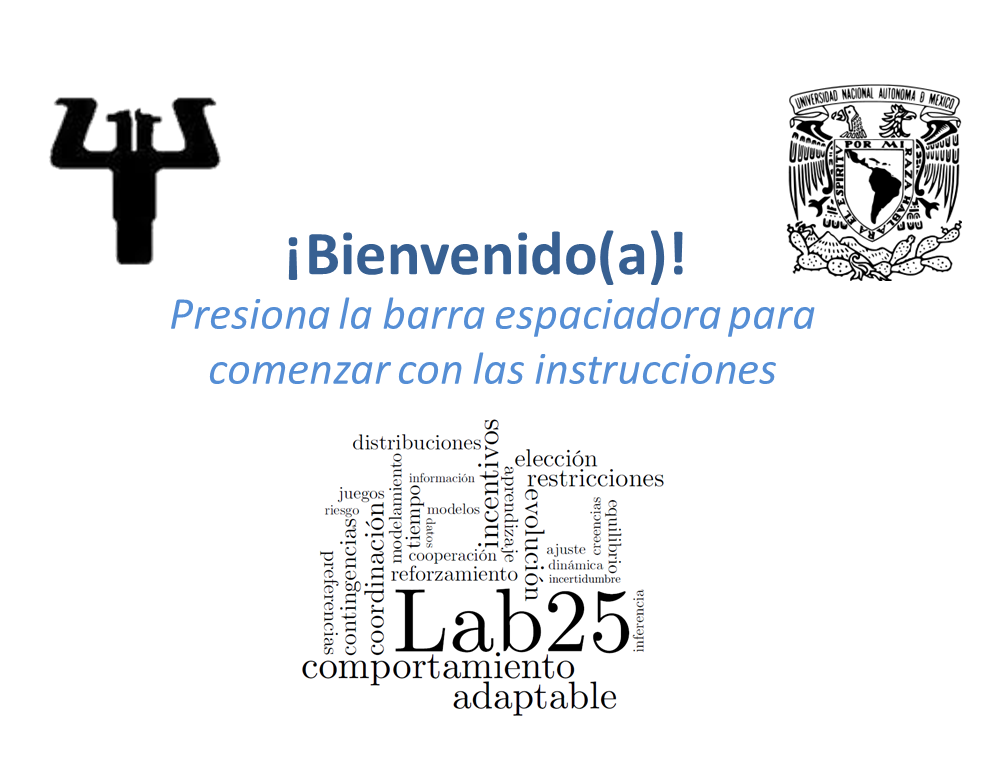
\includegraphics[width=0.95\textwidth]{Figures/Inst_Bienvenido} 
\decoRule
\caption[Pantalla de Bienvenida]{Al entrar al cubículo designado para la realización del experimento, los participantes eran recibidos con un mensaje de bienvenida en la pantalla de la computadora.}
\label{fig:csv}
\end{figure}

\textbf{5. Pantalla con instrucciones adicionales}

\begin{figure}[th]
\centering
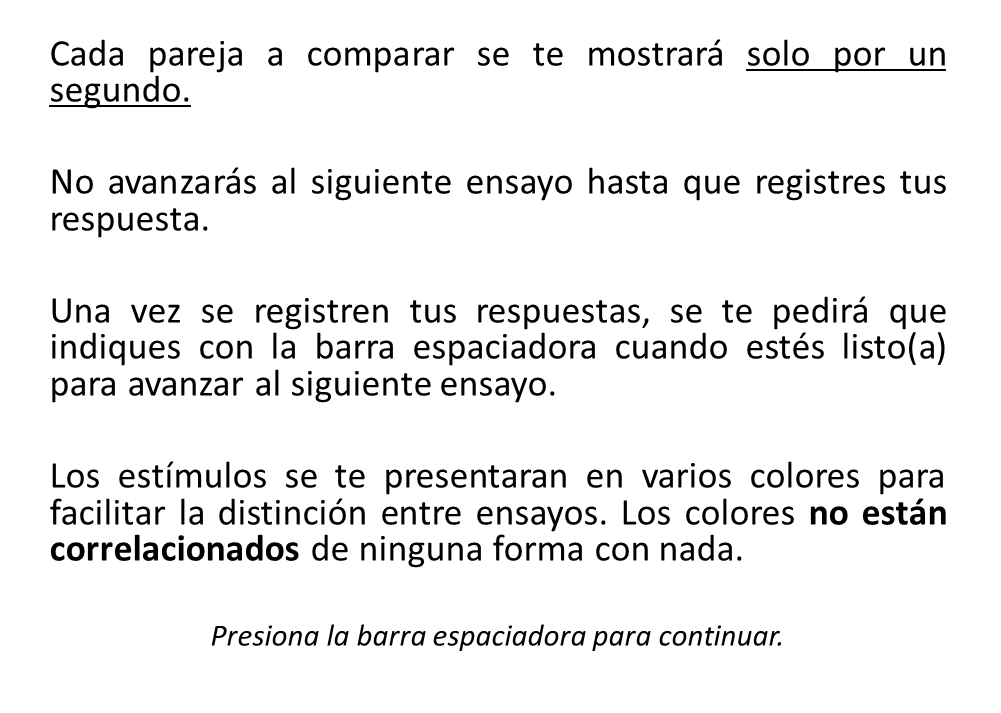
\includegraphics[width=0.95\textwidth]{Figures/Inst_3} 
\decoRule
\caption[Pantalla de Bienvenida]{}
\label{fig:csv}
\end{figure}

\textbf{6. Recordatorio final}

\begin{figure}[th]
\centering
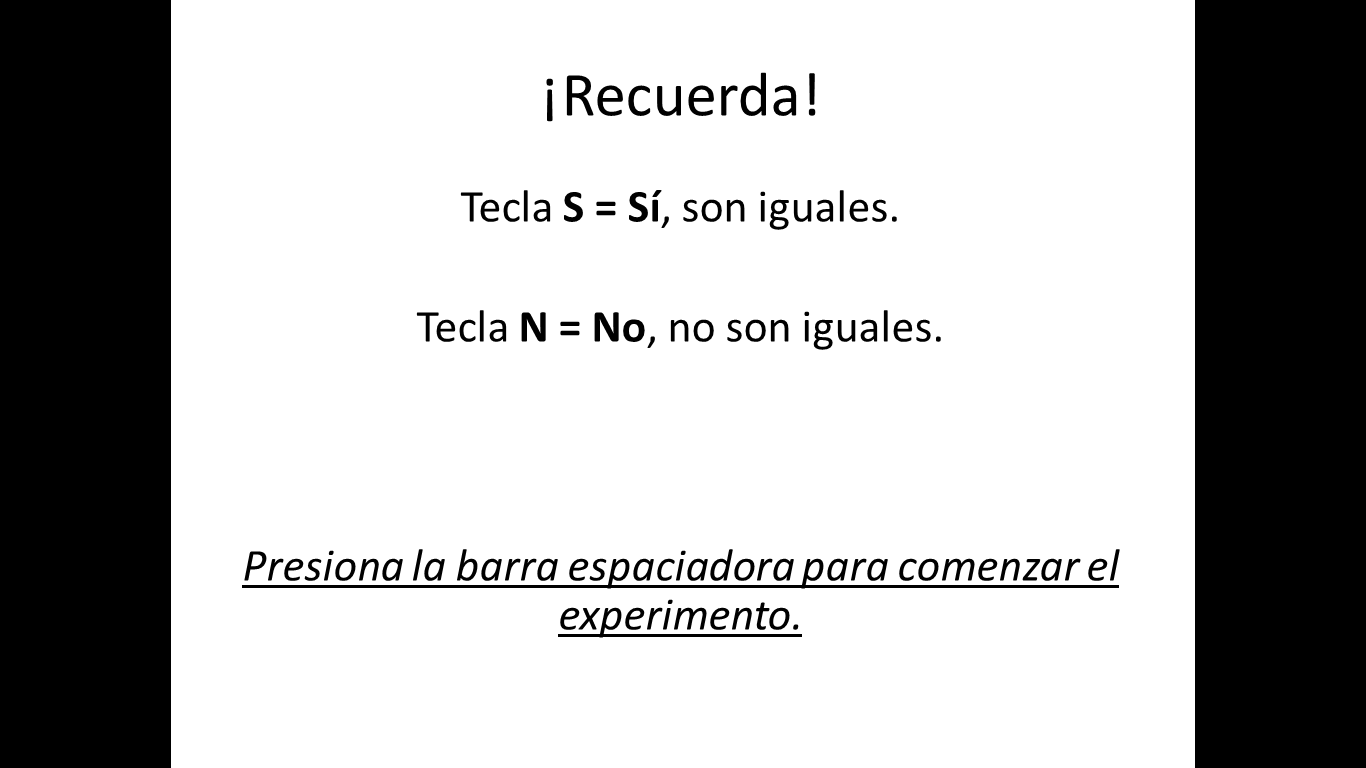
\includegraphics[width=0.95\textwidth]{Figures/Inst_4} 
\decoRule
\caption[Pantalla de Bienvenida]{}
\label{fig:csv}
\end{figure}
